subsubsection{SRS Architecture}\label{sss:calctrainpos}

\begin{itemize}
\item \textbf{SRS High Level Architecture}\\


\begin{figure}[hbtp]
\centering
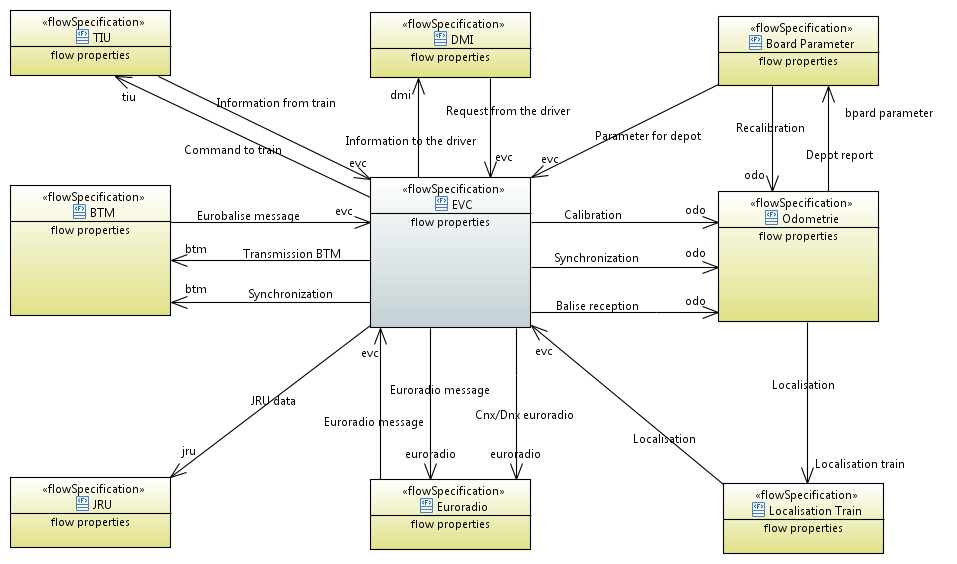
\includegraphics[scale=1]{../images/HighLevelArchitecture.png}
\caption{SRS HighLevel Architecture}
\end{figure}


\begin{enumerate}



\item \textbf{\textit{delDispensableBGs}}: Delete dispensable balise groups\\
The second stage removes balise groups supposed not to be needed any longer from the list of \textit{BGs}.\\
If the number of stored passed linked BGs exceeds the maximum number of eight as specified in subset-26-3.6.2.2.2 c), all BGs astern are deleted.
If only (passed) unlinked BGs are in the list and exceed the number of \textit{cNoOfAtLeast\_x\_unlinkedBGs}, all passed BGs astern to those are removed from the list. 

\item \textbf{\textit{calculateTrainPositionInfo}}: Calculate train position information.\\
This stage take the list of stored BGs and the current odometry values as inputs and steadily provides the current train position. 

\item \textbf{\textit{calculateTrainpositionAttributes}}: Calculate train position attribute information.\\
This stage provides several additional position related attributes that might conveniently be used by subsequent consumers in the architecture. It requires the actual LRBG and the previous LRBG to be assigned external from the list \textit{BGs}. 

\end{enumerate}


\end{itemize}

\subsubsection{Provide Position Report}\label{sss:provposrep}

\begin{figure}[ht]
\centering
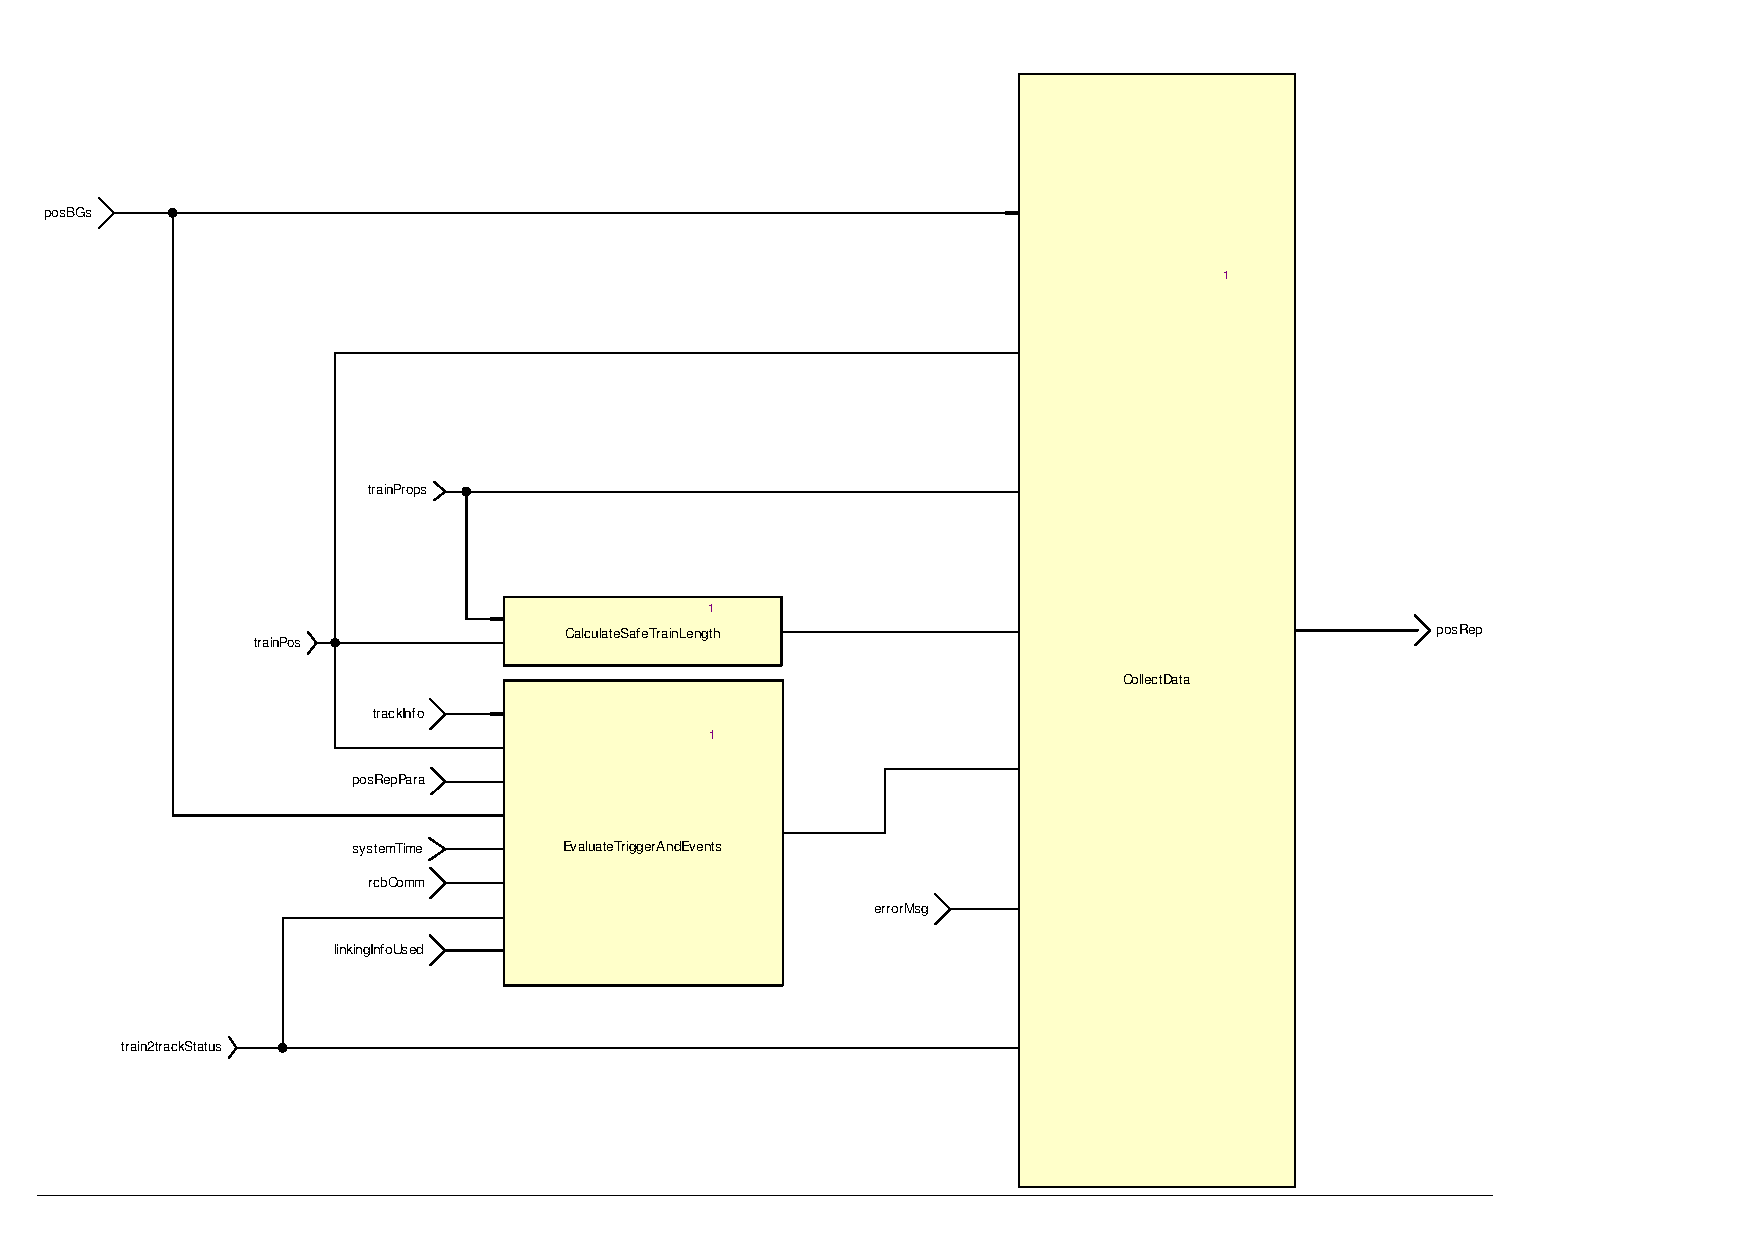
\includegraphics[scale=0.6]{../images/ProvidePositionReport.pdf}
\caption{Structure of component ProvidePositionReport}\label{fig:provideposrep}
\end{figure}

\begin{itemize}
\item \textbf{Short Description of Functionality}\\
This function takes the current train position and generates a position report which is sent to the RBC. The point in time when such a report is sent is determined from event, on the one hand, and position report parameters---which are basically triggers---provided by the RBC or a balise group passed, on the other hand. The functionality is modeled using three operations, as shown in Fig.~\ref{fig:provideposrep}, which are explained below.
\begin{description}
	\item[CalculateSafeTrainLength] Calculates the the safeTrainLength according to Chapt.~3.6.5.2.4/5.
\verb+safeTrainLength = absolute(EstimatedFrontEndPosition - MinSafeRearEnd)+, where
\verb+MinSafeRearEnd = minSafeFrontEndPosition - L_TRAIN+
	\item[EvaluateTriggerAndEvents] Returns a Boolean modeling whether the sending of the next position report is triggered or not. It is the conjunction of the evaluation of all triggers (PositionReportParameters, i.e., Packet 58) and events (see Chapt.~3.6.5.1.4).
	\item[CollectData] In this operation, data of Packet0, \dots, Packet5 and the header is aggregated to a position report.
\end{description}
\item \textbf{Reference to the SRS (or other requirements}\\
Most of the functionality is described in subset 26, chapter~3.6.5.
\item \textbf{Design Constrains and Choices}\\
\begin{enumerate}
	\item The message length (i.e., attribute \verb+L_MESSAGE+) is by default set to 0; the actual value will be set by the Bitwalker/API.
	\item The attribute \verb+Q_SCALE+ is assumed to be constant; that is, all operations using this attribute do not convert between different values of that attribute.
	\item \textit{PositionReportHeader}: The time stamp (i.e., attribute \verb+T_TRAIN+) is not set; this should be done once the message is being sent by the API
	\item \textit{Packet4}: When aggregating the data for this packet, an error message might be overwritten by a succeeding error message. Because the specification only allows to sent one error in one position report, errors are not being stored in a queue, for instance.
	\item \textit{Packet44}: This packet is currently not contained in a position report as it is not part of the kernel functions.
	\item The usage of attributes \verb+D_CYCLOC+ and \verb+T_CYCLOC+ as part of the triggers specified by the position report parameters (i.e., Packet 58 sent by the RBC) may lead to unexpected results if a big clock cycle together with small values for the attributes is used. The cause is that the current model increments at every clock cycle the reference value for the distance and time by at most \verb+D_CYCLOC+ and \verb+T_CYCLOC+, respectively and not a factor of it.
\end{enumerate}
\item \textbf{Open Issues}
\begin{enumerate}
	\item Operation \textit{EvaluateTriggerAndEvents} currently ignores parameters \verb+N_ITER+, \verb+D_LOC+ and \verb+D_LGTLOC+ which allow to specify up to 32 position at which a report has to be sent. The positions are relative to the location of a reference balise group. If the RBC sends packet 58, then it also provides a reference balise group; otherwise, if packet 58 is sent by a balise group, then this balise group serves a the reference balise group. Possible realisation in the model: Extend in the interface posRepPara (i.e., Packet 58) by a \verb+NID_BG+ referring to the reference balise group. Am assumption would be that this BG can be found in the list of passed balise group provided by \textit{CalculateTrainPosition} in Sect.~\ref{sss:calctrainpos}.
	\item The specification requires to store the last eight balise groups for which a position report has been sent (see 3.6.2.2.2.c).
	\item For all reports that contain Packet 1 (i.e., report based on two balise groups), the RBC sends a coordinate system. It is unclear where this has to be stored (i.e., somehow the balise groups have to be stored in a database which has then to be updated), see 3.4.2.3.3.6. Moreover, such a coordination system can be invalid and then has to be rejected (see 3.4.2.3.3.7-8). On a more abstract level, we need to think about the interface between the RBC and the OBU or a proper abstraction thereof.
	\item The decision whether a the report consists of packet 0 or packet 1, which is provided in 3.4.2.3.3, is currently not completely modeled. So far, 3.4.2.3.3.1 has only been modeled, thereby assuming ``the last balise group detected'' is the last balise group and not the LRBG. 3.4.2.3.3.2 is unclear. To model 3.4.2.3.3.4 I need information about the last two valid balise groups and the train running direction. This information can be obtained by adding a memory or this information will be provided by \textit{CalculateTrainPosition} in Sect.~\ref{sss:calctrainpos}. Likewise, also 3.4.2.3.3.5 requires knowledge about the last two valid balise groups.
\end{enumerate}
\end{itemize}

